% Welcome to POS 305 and POS 304 -- Political Inquiry and Political Analysis. This short tutorial is meant to be read in Overleaf ecosystem so that you can see the output in .pdf format and you can see the corresponding code that produces this document. You will also notice notes throughout the code that will not show up in the printed document. This template is set up so that you can copy and paste portions of it to produce your own work. There are examples of tables, figures, and lists that you will eventually need for your papers. The paper is also organized into sections that will help you when it comes time to producing longer papers. 

% When starting a project, you must first tell LateX the type of document you will be using. Here we will be using the article document and we will signify that by telling LateX that with the \documentclass{} command and designating "article" as the type of document we will be producing.
\documentclass[10pt]{article}

% Like other programs, you must first give a set of instructions so that Latex knows what you are referring to throughout the document when you tell it to do something. In order to do this, typically you will "load" a series of packages into Latex. Sometimes you will know ahead of time which packages you will use. Other times you will realize later that you want to do someting in LateX that requires adding a new package. You can add as many packages as you want, so long as the packages don't contradict another package. Overleaf will prompt you any time there is a coding or command error. Below is the list of packages that I am instructing LateX to install prior to beginning my document. So far as I know, it does not matter how many packages you load into your Latex code. It may compile a bit slower, but unless you have an extremely complex document, you will not notice. For now, I am adding as many packages as possible. Don't worry about what package does what. Just get the hang of what we are trying to do. 

\usepackage{xspace}
\usepackage[utf8]{inputenc}
\usepackage{float}
\usepackage{url} 
\usepackage{ulem}
%\usepackage{geometry}
\usepackage{graphicx}
\usepackage{titling}
\usepackage{caption} %allows captions for graphics
\captionsetup[table]{justification=centering, singlelinecheck=false}  % For main caption
\usepackage[nottoc]{tocbibind} %adds the bibliography to the table of contents
\usepackage{subcaption} %allows subcaption for multiple images in one graphic
\usepackage{booktabs}
\usepackage{hyperref}
\usepackage{amsmath}
\usepackage{graphicx}
\usepackage{rotating}
\usepackage{booktabs}
\usepackage[margin=1in]{geometry}
\usepackage{threeparttable}
\usepackage[most]{tcolorbox}
\usepackage{fancybox} % for \fbox
\newcommand{\R}{\texttt{R}}
\usepackage{lipsum}  
\usepackage{cmbright}

\usepackage[style=apa, backend=biber]{biblatex}
\DeclareLanguageMapping{american}{american-apa}
\usepackage{csquotes}
\addbibresource{references.bib}
\usepackage[hyphens]{url}
\sloppy
\setlength{\bibitemsep}{1em}  % Adjust spacing between items


% When using any document class, there are fields you can designate that will show up throughout your document. For instance, using the "article" documentclass, you can designate a title, author, and date. This information will show up whenever you tell Latex to "print" it. 

\title{NAU POS \LaTeX{} Template} % Delete "template" and add the name of the class here. 
\author{Stephen A. Nu\~no} %delete the name and add your name here
\date{\today}

% Below I am using a package called "fancyhdr" so that I can print a header and footer at the bottom of my first page. I separated this package just so you can see how this specific package works within the document to the right. 

 \usepackage{fancyhdr}
  \setlength{\headheight}{12.49998pt}
\fancypagestyle{plain}{%  the preset of fancyhdr 
    \fancyhf{} % clear all header and footer fields
    %\fancyfoot[R]{
\includegraphics[width=2.5cm]{Images/NAU_ctr_282_3514_150.png}}
    \fancyfoot[R]{\theauthor}
    \fancyfoot[L]{\thedate}
    \fancyhead[L]{NAU POS \LaTeX{} Template}
    %\fancyhead[R]{\theauthor}
    \fancyhead[R]{
\includegraphics[width=2.5cm]{Images/NAU_ctr_282_3514_150.png}}

}
% The next few lines are simply creating some space above the footer, so that it does not look crowded. You can experiment by cutting out this command and hitting the "recompile" button, to see the difference in look. 

\makeatletter
\def\@maketitle{%
  \newpage
  \null
  \vskip 1em%
  \begin{center}%
  \let \footnote \thanks
    {\LARGE \@title \par}%
    \vskip 1em%
    %{\large \@date}%
  \end{center}%
  \par
  \vskip 1em}
\makeatother

% OK, now lets begin our document! We need to tell LateX this with the \begin command. Note that when you begin a command, Overleaf will intuitively guess what command you may want to use. It will suggest different codes in a drop down menu that you can go down to and hit the Enter key so you do not have to type it all. I will also add the brackets, where you can enter any options, if they are available. 

\begin{document}

\maketitle % Note that this command is telling LateX to place the title of the document here. Recall earlier that we designated this title earlier in the code. 

% I created a non-descript table so that you can add your name, student id and date. Note that I am using the \today command here. This is telling Latex to add whatever today's date is by default. This can be useful, but you can also delete that and add the actual date you want shown in your document. 

\noindent\begin{tabular}{@{}ll}
    Name: & \theauthor\\
     Student ID: &  \#XXXXXXXX\\
     Date: & \today
\end{tabular}

% OK, we are going to start by telling LateX we want to begin a new section. Here we are using the \section command. Note the astericks (*) next to the command. The astericks is useful because we do not want Latex to number this section. You can delete the astericks and recompile to see what a numbered section looks like. Also, you will notice that when you create a new section, the File outline window on the bottom left of your Overleaf ecosystem lists your sections and subsections. You can click on the section if you want to go directly to that section. 

\section*{Introduction to \LaTeX{}} %note the little asterick * after each section. If you do not include the asterick, LaTeX will think you want each section and subsection numbered. You may choose to number your sections, but for now you do not need to. 

Welcome to POS 304 and 305 -- Political Inquiry and Political Analysis. This short tutorial is meant to be read in the Overleaf ecosystem so that you can see the output in .pdf format and you can see the corresponding code that produces this document. You will also notice notes throughout the code that will not show up in the printed document. This template is set up so that you can copy and paste portions of it to produce your own work. There are examples of tables, figures, and lists that you will eventually need for your assignment papers. This document is also organized into sections that will help you when it comes time to producing longer papers. %Notice how this section is associated with "line 98". You do not need to hit return, LaTeX will automatically format each paragraph as a single thought. But you will need to skip a line to tell LaTeX to start a new paragraph, which as you can see by the output, is identend. 

 You are expected to use this template for major papers this semester. This is a program called \LaTeX, a typesetting program that is widely used in academia to produce professional looking documents. \LaTeX{} is essential for academic students because it produces high--quality, professional looking documents, especially for papers with complex formatting, equations, citations, and tables. Unlike Microsoft Word or Google Docs, which are WYSIWYG (what you see is what you get) word processors, \LaTeX{} separates content from formatting, ensuring consistent structure and style throughout your work. It is especially valuable in disciplines like mathematics, engineering, and the social sciences, where clarity and precision are critical. While Word and Google Docs are useful for collaboration and quick edits, they struggle with advanced typesetting and large documents. Learning LaTeX equips students with a powerful tool for academic publishing and scholarly communication. 

The \LaTeX{} programming language is very simple, but it will take some getting used to because it forces you to be intentional about how you present your work. It not only produces a better looking product, but it forces you to be more logical about the structure of what you are writing. Below are some examples you will use throughout the semester to produce your work. We will begin with very simple output, and eventually you will produce your entire political analysis using this program. In addition to \LaTeX{}, you will need to use the statistical program called \R{} (POS 305 students only) and a reference management system called Zotero. Together, these programs will give you the power to present your analysis the same way that academics do. 

\newpage %This command tells LaTeX to start a new page, like "page break" in Microsoft Word.
\section*{First things first}
\LaTeX will compile all sorts of documents, figures, photos, .pdfs, etc. into a single document. In order for to do so, however, you need to upload those files into the library you see on the top left frame of the Overleaf program. Make sure you have your library window set up the way I have it so that this goes as smoothly as possible. Once you get the hang of Overleaf, you can organize your files any way you like.  

\begin{figure} [H] % opens the figure environment. the '[H]' forces the image to be Here
    \centering % puts the image in the horizontal centre of the page
    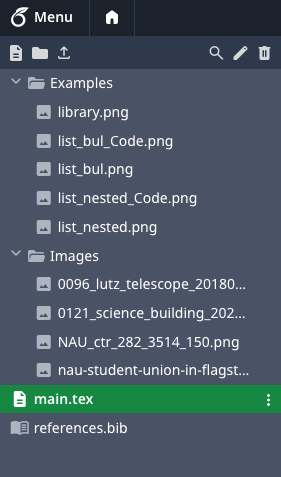
\includegraphics[width = 8cm]{Examples/library.png} %this tells latex what graphics to include. I put this image in the 'Examples' folder to aid file management, hence the Examples/ before the file name. The width bit before allows you to alter the width of the image. It is also possible to use scale as well as using equations with the textwidth to make it say half the text width. Here, I've set the width of the image to 8cm's wide.
\end{figure}

\section*{Text}
As you can see, \LaTeX{} ``looks" better, but it functions a little different than a standard word processor. You can still use \textit{italics}, and you can \textbf{bold} your text, but you will need to do this intentionally by using the correct code. Fortunately, Overleaf gives you an interface that allows you to do this by highlighting what you want to emphasize and then clicking on the corresponding icon at the top. To \uline{underline}, you will need to code it out manually. You can also cite your work very easily by uploading your bibliography ahead of time as a ``bib file" and then using \LaTeX{} to insert your citations \parencite{cadena_paradoxical_2023}. We will look at citations in a bit.

\section*{Tables}
When beginning a table, you must identify the number of columns and how you want the contents of each column to be justified, left (l), right (r) or centered (c). In Table \ref{tab:wide} you can see that the table is labeled "wide". When labeling your tables, you can refer to them throughout the text so that the reader can click on the link and go directly to the table in the final product. For instance, you can refer to Table \ref{tab:regress} so you can click on the hot link and go to that table in the pdf, similar to citations. 

Use the table and tabular commands for basic tables --- see Table \ref{tab:wide}, for a simple example. \href{http://tablesgenerator.com}{TablesGenerator.com} is a handy tool for designing tables and generating the LaTeX code, which you can copy and paste into your article here.

Below are three examples of a basic tables you will need to create in class. First, a table with a simple list in Table \ref{tab:wide}, second a more complex table that lists items with multiple rows and columns in Table \ref{tab:wide}, and finally a regression table down in Table \ref{tab:regress}. 

\subsection*{Simple Tables}

I am presenting a number of examples using the tabular environment. The codes below give the basic structure of your tables. You can use the codes for the tables below or you are free to use an AI agent, such as ChatGPT, Claude, or Pilot to help you. While those AI tools are helpful, you need to know what to ask in order to take advantage of AI assistance. 

\vspace{5mm}
\begin{center}
\begin{tabular}{ l c r }
  1 & 2 & 3 \\
  4 & 5 & 6 \\
  7 & 8 & 9 \\
\end{tabular}
\end{center}

\vspace{5mm}
% The following table is the same as above, but the code below adds some vertical lines: 
\vspace{5mm}

\begin{center}
\begin{tabular}{ l | c | r }
  1 & 2 & 3 \\
  4 & 5 & 6 \\
  7 & 8 & 9 \\
\end{tabular}
\vspace{5mm}
\end{center}
%Without specifying width for last column:



\begin{center}
\begin{tabular}{llr}
\hline
\multicolumn{2}{c}{Item} \\
\cline{1-2}
Animal    & Description & Price (\$) \\
\hline
Gnat      & per gram    & 13.65      \\
          & each        & 0.01       \\
Gnu       & stuffed     & 92.50      \\
Emu       & stuffed     & 33.33      \\
Armadillo & frozen      & 8.99       \\
\hline
\end{tabular}
\end{center}
\vspace{5mm}

\begin{center}
\begin{tabular}{lr}
\toprule %creates a top line 
Item & Quantity \\
\midrule %creates a line above the items and below the header of the table
Widgets & 42 \\
Gadgets & 13 \\
\bottomrule %creates a line below the last item
\end{tabular} 
\end{center}
\vspace{5mm}

\subsection*{Minor Adjustments to Tables}
The tabular environment can vastly change how your table looks if you are missing some simple instructions. Below are two tables with minor adjustments that illustrates how tables can look much better with some simple commands. The two tables below are the same with the exception of the simple instruction to limit the size of the last column.

\begin{center}
    \begin{tabular}{| l | l | l | l |}
    \hline
    Day & Min Temp & Max Temp & Summary \\ \hline
    Monday & 11C & 22C & A clear day with lots of sunshine.
    However, the strong breeze will bring down the temperatures. \\ \hline
    Tuesday & 9C & 19C & Cloudy with rain, across many northern regions. Clear spells 
    across most of Scotland and Northern Ireland, 
    but rain reaching the far northwest. \\ \hline
    Wednesday & 10C & 21C & Rain will still linger for the morning. 
    Conditions will improve by early afternoon and continue 
    throughout the evening. \\
    \hline
    \end{tabular}
\end{center}
\vspace{5mm}

%With width specified:
\begin{center}
    \begin{tabular}{ | l | l | l | p{5cm} |}
    \hline
    Day & Min Temp & Max Temp & Summary \\ \hline
    Monday & 11C & 22C & A clear day with lots of sunshine.  
    However, the strong breeze will bring down the temperatures. \\ \hline
    Tuesday & 9C & 19C & Cloudy with rain, across many northern regions. Clear spells 
    across most of Scotland and Northern Ireland, 
    but rain reaching the far northwest. \\ \hline
    Wednesday & 10C & 21C & Rain will still linger for the morning. 
    Conditions will improve by early afternoon and continue 
    throughout the evening. \\
    \hline
    \end{tabular}
\end{center}
\vspace{5mm}

\subsection*{More Complex Tables}
Below is a more complex table. You can use this as a template for a multi-column table. 

\begin{table}[H]
\centering %centers the table
\caption{This is an example of a more complex table.}
\label{tab:wide}
\begin{tabular}{l c l l r} %when beginning a table, you must identify the number of columns and how you want the contents of each column to be justified, left (l), right (r) or centered (c) 
Speed (mph) & Driver          & Car                        & Engine    & Date     \\
\toprule
407.447     & Craig Breedlove & Spirit of America          & GE J47    & 8/5/63   \\
413.199     & Tom Green       & Wingfoot Express           & WE J46    & 10/2/64  \\
434.22      & Art Arfons      & Green Monster              & GE J79    & 10/5/64  \\
468.719     & Craig Breedlove & Spirit of America          & GE J79    & 10/13/64 \\
526.277     & Craig Breedlove & Spirit of America          & GE J79    & 10/15/65 \\
536.712     & Art Arfons      & Green Monster              & GE J79    & 10/27/65 \\
555.127     & Craig Breedlove & Spirit of America, Sonic 1 & GE J79    & 11/2/65  \\
576.553     & Art Arfons      & Green Monster              & GE J79    & 11/7/65  \\
600.601     & Craig Breedlove & Spirit of America, Sonic 1 & GE J79    & 11/15/65 \\
622.407     & Gary Gabelich   & Blue Flame                 & Rocket    & 10/23/70 \\
633.468     & Richard Noble   & Thrust 2                   & RR RG 146 & 10/4/83  \\
763.035     & Andy Green      & Thrust SSC                 & RR Spey   & 10/15/97\\
\bottomrule
\end{tabular}

\vspace{2mm}
\caption*{\textit{Note:} This is a caption note that is not "counted", like Table 
\ref{tab:regress}, Table \ref{tab:table}, etc. are.}
\end{table}

\newpage
\subsection*{Cross-tabulation Table}
\begin{table}[ht]
\centering
\caption{Column Percentages by Social Class and EV Ownership (Q9 × Q24)}
\label{tab:q9_q24_colpct}
\begin{tabular}{lccc}
\toprule
Social Class & Yes & No & I do not know \\
\midrule
Upper class        & 25\% & 1\% & 0\% \\
Upper-middle class & 34\% & 13\% & 2\% \\
Middle class       & 31\% & 39\% & 43\% \\
Working class      & 9\%  & 36\% & 36\% \\
Poor               & 1\%  & 10\% & 18\% \\
\midrule
Total              & 100\% & 100\% & 100\% \\
\bottomrule
\end{tabular}
\vspace{2mm}
\caption*{\textit{Note:} This is a caption note that is not "counted," like Table captions.}
\end{table}

\newpage
\subsection*{Regression Table}

\begin{table*}[htbp!] \centering \footnotesize
  \caption{This is an example of a regression table} 
  \label{tab:regress} 
\begin{tabular}{@{\extracolsep{5pt}}lcccc} 

 & \multicolumn{4}{c}{\textsl{Dependent variable: $log(Dependent Variable_{t-1} + 1)$}} \\ 
\cline{2-5} 
\\[-1.8ex] & (1) & (2) & (3) & (4) \\ 
\hline \\[-1.8ex] 
  Variable q  & $-$0.512 & $-$0.674 & $-$0.421 & $-$0.374 \\ 
  & (0.510) & (0.525) & (0.517) & (0.537) \\ 
  Variable 2 & 1.108$^{***}$ & 0.798$^{***}$ & 0.784$^{***}$ & 0.703$^{**}$ \\ 
  & (0.288) & (0.283) & (0.275) & (0.288) \\ 
  Variable 3  & 0.200 & 0.202 & 0.304$^{**}$ & 0.285$^{**}$ \\ 
  & (0.138) & (0.139) & (0.139) & (0.138) \\ 
  Variable 4 &  & $-$0.766$^{***}$ & $-$1.036$^{***}$ & $-$0.982$^{***}$ \\ 
  &  & (0.254) & (0.255) & (0.251) \\ 
  Variable 5 &  & 0.120 & 0.232$^{*}$ & 0.260$^{*}$ \\ 
  &  & (0.127) & (0.134) & (0.138) \\ 
  Variable 6 &  & 0.341$^{***}$ & 0.395$^{***}$ & 0.357$^{***}$ \\ 
  &  & (0.071) & (0.072) & (0.072) \\  
  Variable 7 &  &  & 0.232$^{***}$ & 0.189$^{***}$ \\ 
  &  &  & (0.034) & (0.036) \\ 
  Variable 8 &  &  & 0.253$^{***}$ & 0.206$^{***}$ \\ 
  &  &  & (0.037) & (0.042) \\ 
  Variable 9 &  &  & 0.060$^{***}$ & 0.051$^{***}$ \\ 
  &  &  & (0.008) & (0.009) \\ 
  Variable 10 &  &  & $-$0.018$^{***}$ & $-$0.012$^{*}$ \\ 
  &  &  & (0.007) & (0.007) \\ 
  Variable 11 &  &  &  & 0.329$^{***}$ \\ 
  &  &  &  & (0.125) \\ 
   Constant & 0.275$^{***}$ & 0.946$^{***}$ & $-$2.334$^{***}$ & $-$1.017$^{**}$ \\ 
  & (0.056) & (0.298) & (0.439) & (0.475) \\ 
\hline \\[-1.8ex] 
Obs. & 32,658 & 32,658 & 32,658 & 28,200 \\ 
Adj. R$^{2}$ & 0.371 & 0.374 & 0.389 & 0.429 \\ 
F Stat. & 2,756.800$^{***}$  & 1,949.369$^{***}$  & 1,485.940$^{***}$  & 1,058.683$^{***}$  \\ 
\hline \\[-1.8ex] 
\textsl{Note:}  & \multicolumn{4}{l}{$^{*}$p$<$0.1; $^{**}$p$<$0.05; $^{***}$p$<$0.01} \\ 
\end{tabular} 
\end{table*}  

\newpage

\section*{Images}
As you can see in the code for this section, images are enclosed within a figure environment. \LaTeX{} will sometimes try to position the figure/table/image where it thinks it fits best into the text. This can be frustrating, since you may disagree with \LaTeX{}, but that is fine. To disagree there are many options. I tend to force \LaTeX{} to put the figure where I have put the figure environment in my code as this often allows me better control of the image positioning. This is done using [H] on the same line as the \verb+\begin{figure}+ command. There are other places you can force the figure to be placed and these are covered in \url{https://www.overleaf.com/learn/latex/Positioning_images_and_tables}. Please see the annotated code for this chapter for an example.

\begin{figure} [H] % opens the figure environment. the '[H]' forces the image to be Here
    \centering % puts the image in the horizontal centre of the page
    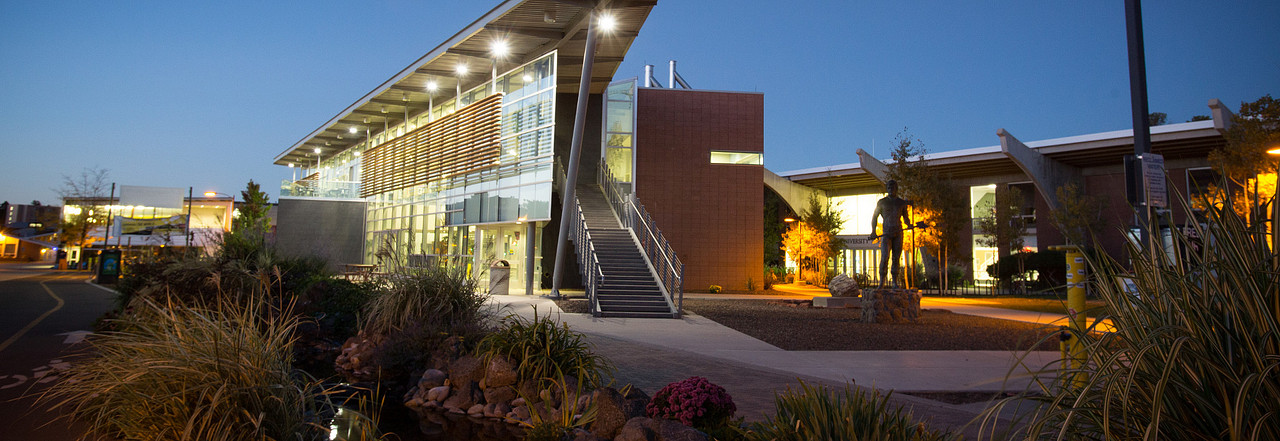
\includegraphics[width = \textwidth]{Images/nau-student-union-in-flagstaff.jpeg} %this tells latex what graphics to include. I put my images in an 'Images' folder to aid file management, hence the Images/ before the file name. the width bit before allows you to alter the width of the image. It is also possible to use scale as well as using equations with the textwidth to make it say half the text width.
    \caption{University Union \copyright Northern Arizona University} % this prints the caption below the figure
    \label{fig:union} % this internally labels the figure for future referencing.
\end{figure}

\newpage
\section*{Multiple Images}

It is also possible to put multiple images next to each other to compare them. Please look at the code for the following images to see how this is done. Below are images where one is above the other, one is next to the other, and one is next to the other with both images within a gray box. You can see how the images are labled, and how both images are counted as one "Figure". Similar to the tables, you can label them so that you can refer them throughout the text, and you can refer to each particular picture within the figure, such as Figure \ref{fig:kitt} or Figure \ref{fig:kittbldg1}

\begin{figure} [H]
\centering
\begin{subfigure}{1\textwidth}
  \centering
  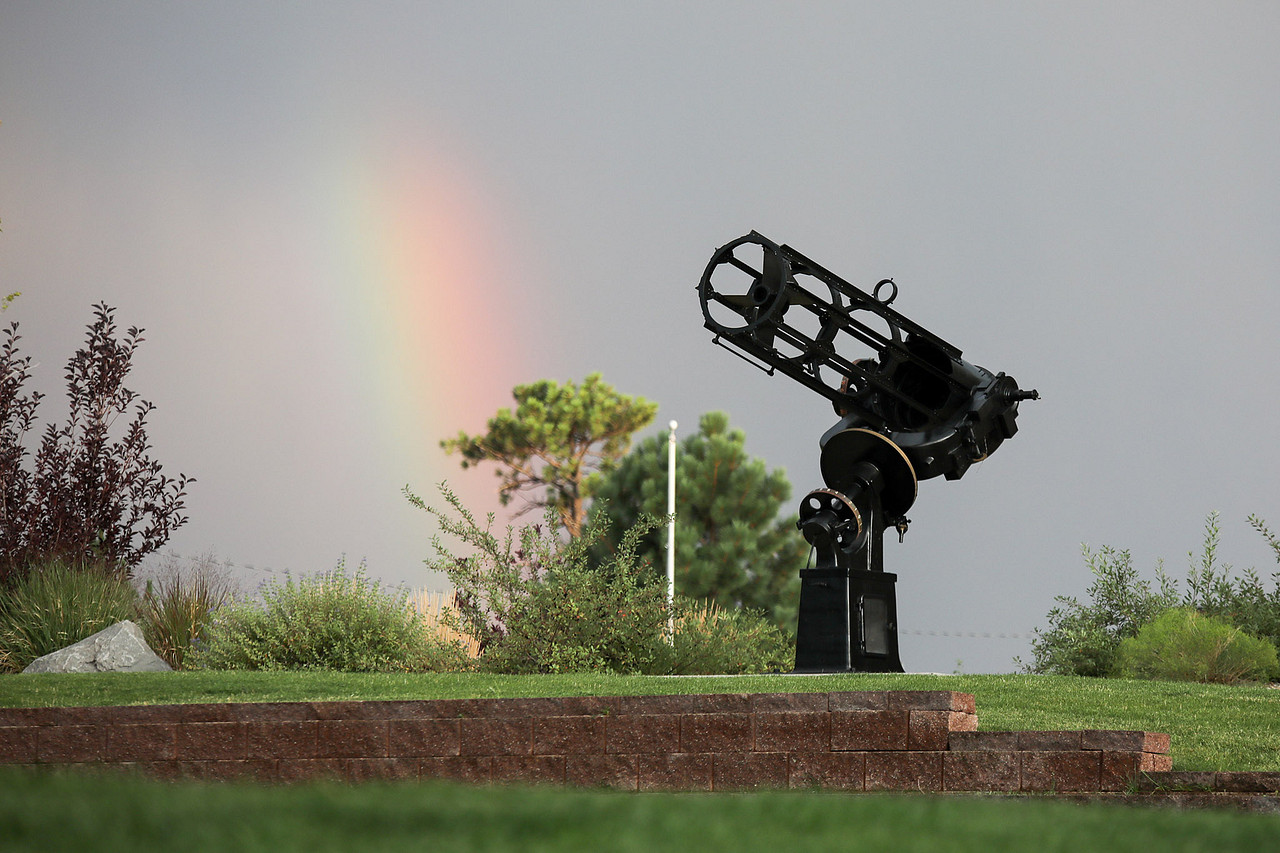
\includegraphics[width=.45\linewidth]{Images/0096_lutz_telescope_20180814.jpeg}
  \caption{Lutz Telescope, \copyright Northern Arizona University}
  \label{fig:lutz}
\end{subfigure}
\begin{subfigure}{1\textwidth}
  \centering
  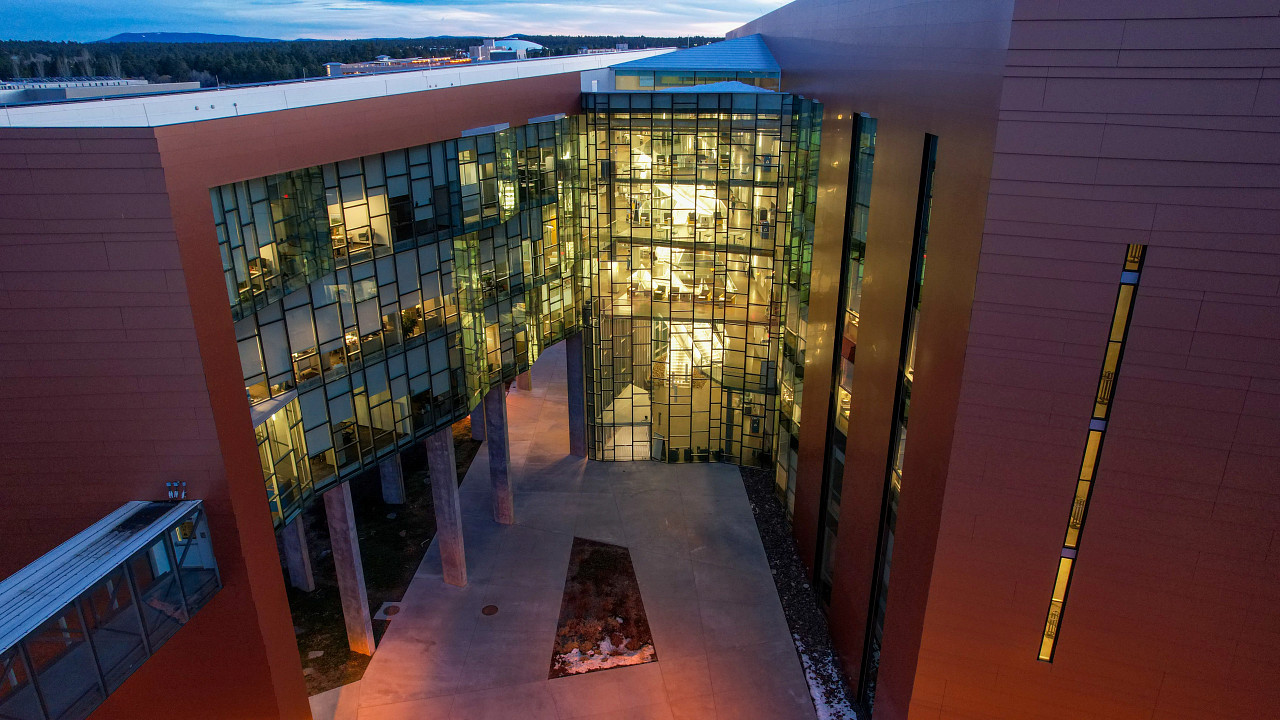
\includegraphics[width=.45\linewidth]{Images/0121_science_building_20220113.jpeg}
  \caption{Kitt Science Bldg., \copyright Northern Arizona University}
  \label{fig:KempfT}
\end{subfigure}
\caption{Multiple Images, one above the other}
\label{fig:kitt}
\end{figure}

\begin{figure}[H]
\centering
\begin{subfigure}{0.48\textwidth}
  \centering
  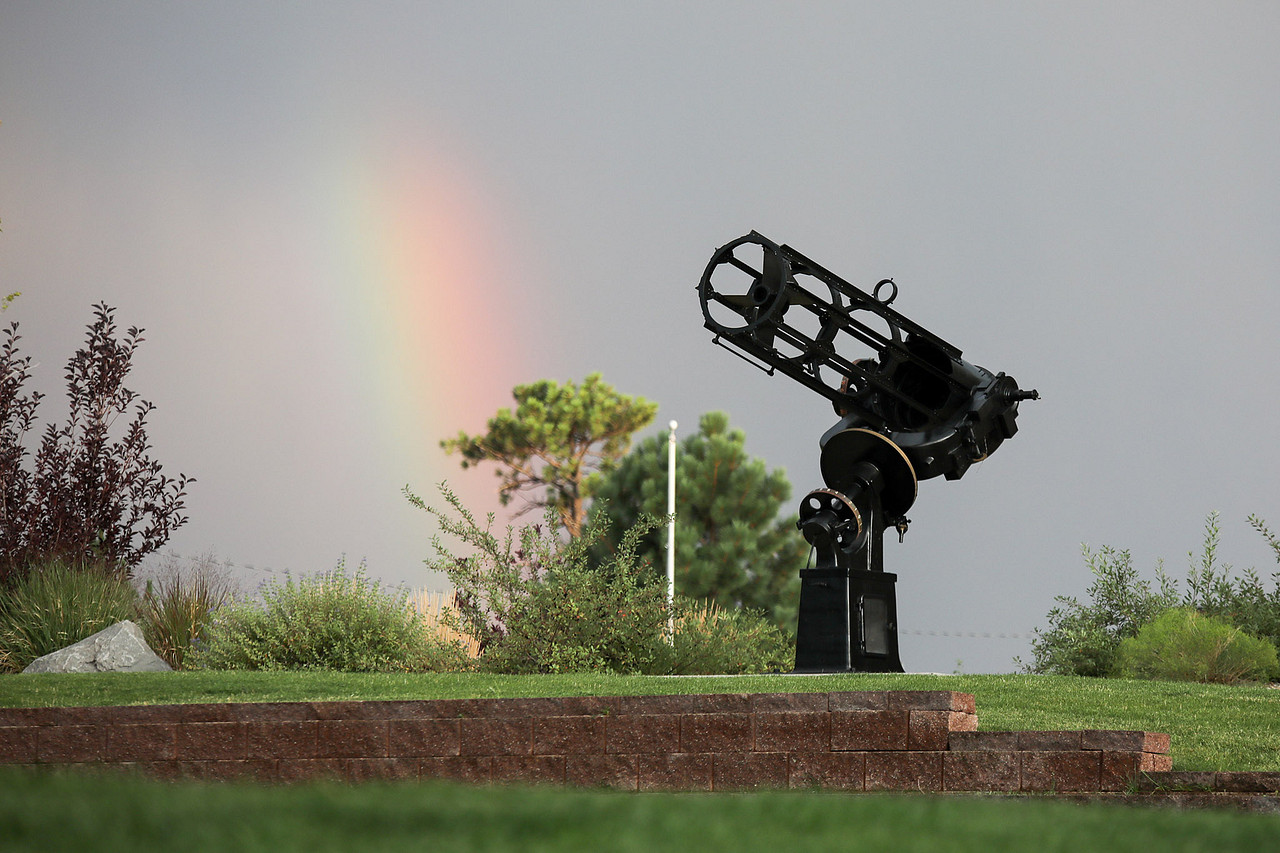
\includegraphics[width=\linewidth]{Images/0096_lutz_telescope_20180814.jpeg}
  \caption{Lutz Telescope, \copyright Northern Arizona University}
  \label{fig:lutz1}
\end{subfigure}
\hfill
\begin{subfigure}{0.48\textwidth}
  \centering
  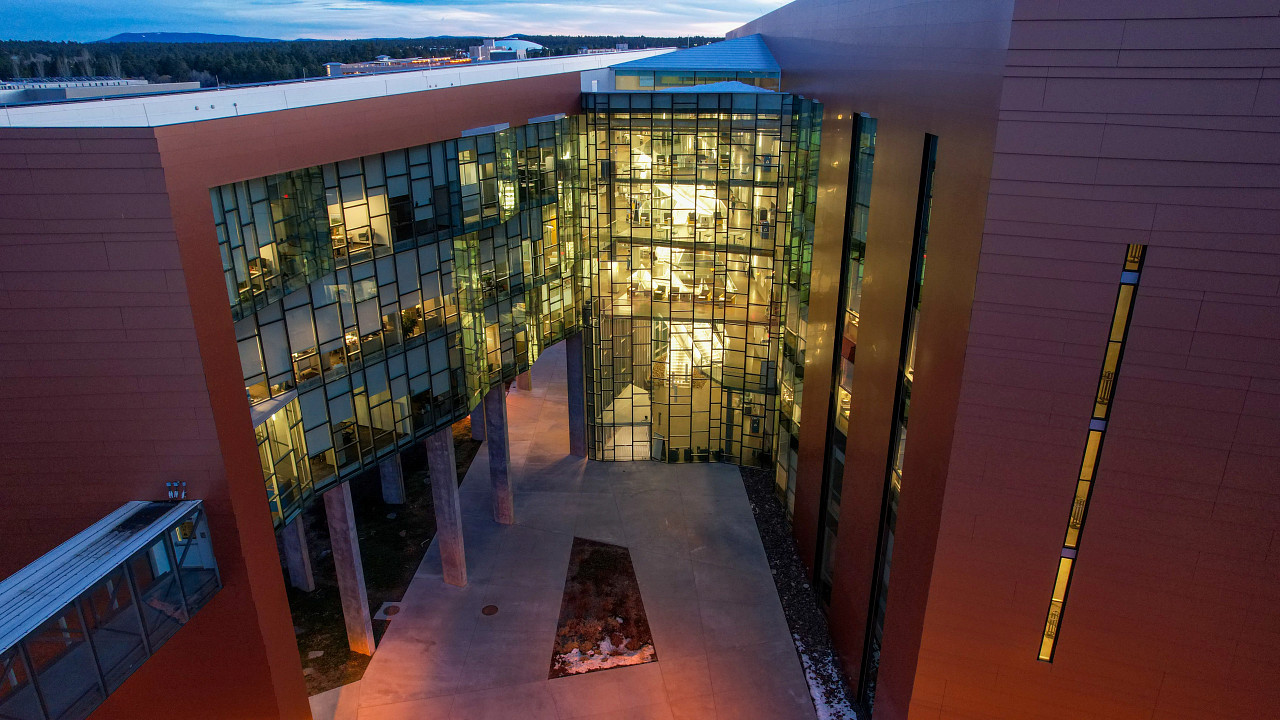
\includegraphics[width=\linewidth]{Images/0121_science_building_20220113.jpeg}
  \caption{Kitt Science Bldg., \copyright Northern Arizona University}
  \label{fig:kittbldg1}
\end{subfigure}
\caption{Multiple Images side by side}
\label{fig:side}
\end{figure}


\begin{tcolorbox}[colframe=black, boxrule=0.5pt, sharp corners, enhanced]
\begin{figure}[H]
\centering
\begin{subfigure}{0.48\textwidth}
  \centering
  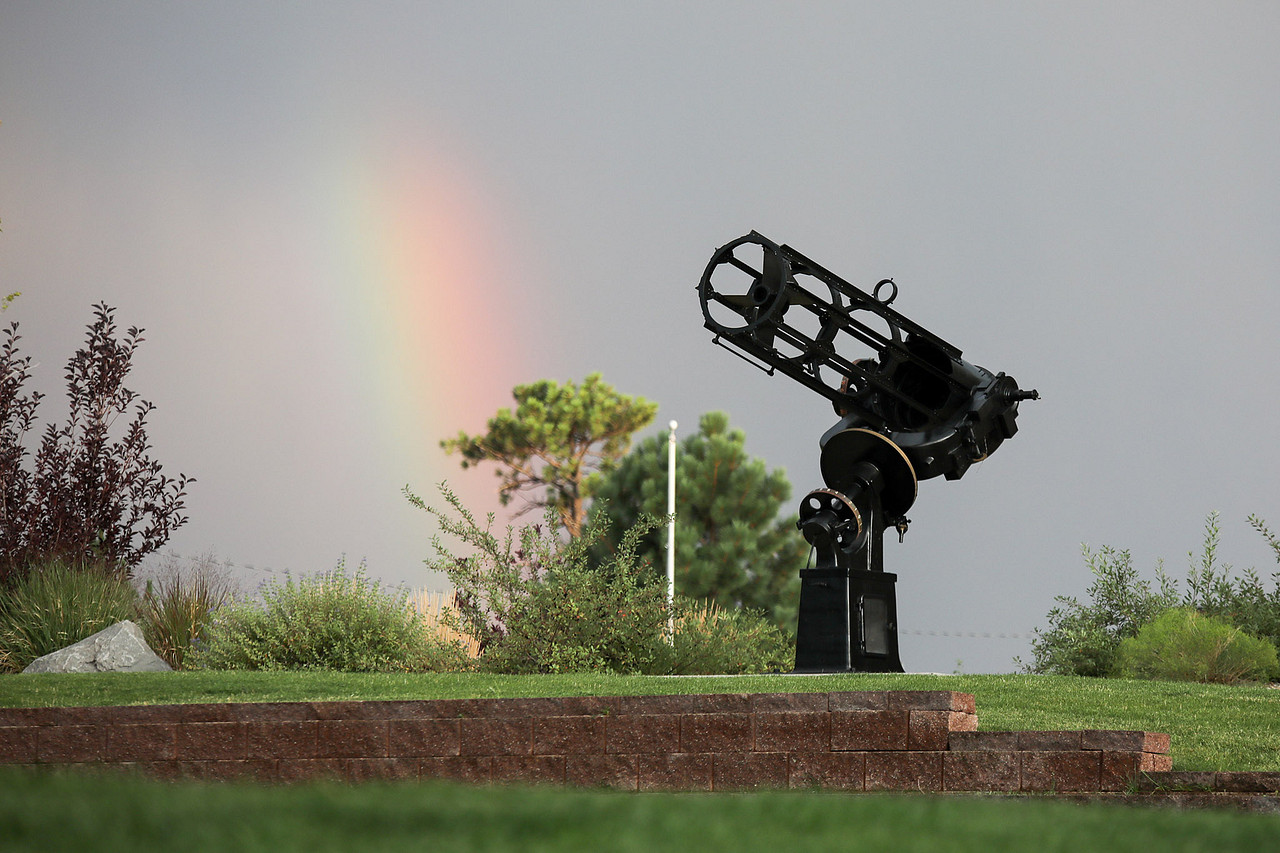
\includegraphics[width=\linewidth]{Images/0096_lutz_telescope_20180814.jpeg}
  \caption{Lutz Telescope, \copyright Northern Arizona University}
  \label{fig:lutz2}
\end{subfigure}
\hfill
\begin{subfigure}{0.48\textwidth}
  \centering
  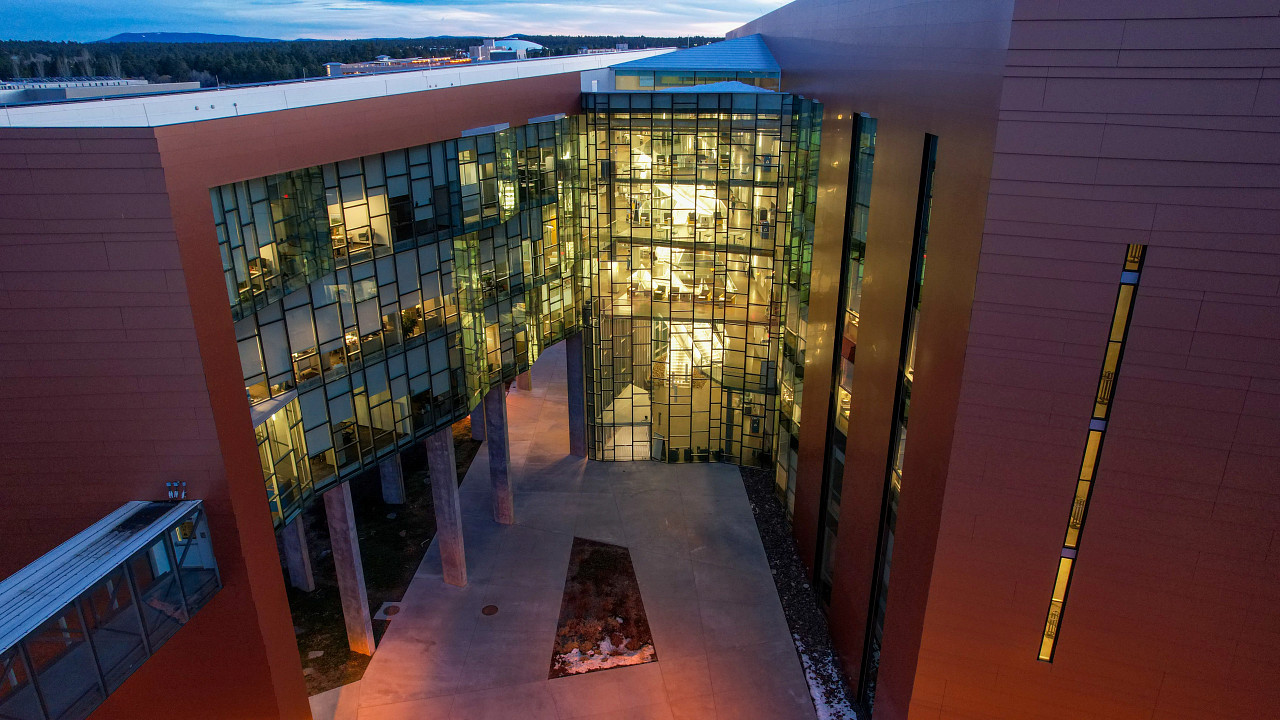
\includegraphics[width=\linewidth]{Images/0121_science_building_20220113.jpeg}
  \caption{Kitt Science Bldg., \copyright Northern Arizona University}
  \label{fig:kittbldg2}
\end{subfigure}
\caption{Multiple images side by side that are placed within a gray box}
\label{fig:box}
\end{figure}
\end{tcolorbox}

\newpage
\section*{Lists}
You often need to produce lists of things. \LaTeX{} has a list environment that is easy to use once you get the hang of it. 

You can make lists with automatic numbering using the \verb|\enumerate| command \dots

\begin{enumerate}
\item Like this,
\item and like this,
\item and also this.
\end{enumerate}

You can also nest lists within lists, such as below. The code for the nested lists and the product of the code are below, inserted as two figures side-by-side with a line between the two figures.

\begin{figure}[ht]
\centering

\begin{subfigure}[t]{0.3\textwidth}
  \raggedright
  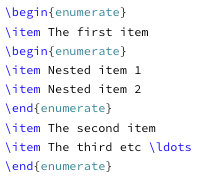
\includegraphics[width=\linewidth]{Examples/list_nested_Code.png}
  \caption{\LaTeX Code}
  \label{fig:list_ex1.1}
\end{subfigure}
%\hfill
\vrule width 1pt
%\hfill
\begin{subfigure}[t]{0.3\textwidth}
  \raggedleft
  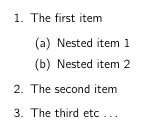
\includegraphics[width=\linewidth]{Examples/list_nested.png}
  \caption{Ouput}
  \label{fig:list_ex1.2}
\end{subfigure}

\caption{Nested Numbered List}
\label{fig:list_ex1}
\end{figure}
\vspace{1cm}
You can do this with bullet points, as well, using the \verb|\itemize| command \dots 

\begin{figure}[ht]
\centering

\begin{subfigure}[t]{0.3\textwidth}
  \raggedright
  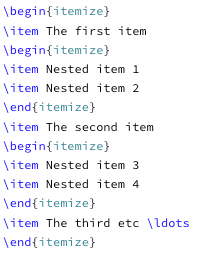
\includegraphics[width=\linewidth]{Examples/list_bul_Code.png}
  \caption{\LaTeX Code}
  \label{fig:list_ex2.1}
\end{subfigure}
%\hfill
\vrule width 1pt
%\hfill
\begin{subfigure}[t]{0.3\textwidth}
  \raggedleft
  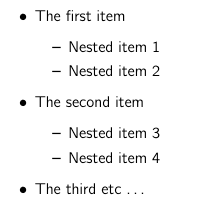
\includegraphics[width=\linewidth]{Examples/list_bul.png}
  \caption{Ouput}
  \label{fig:list_ex2.2}
\end{subfigure}

\caption{Nested Bulleted List}
\label{fig:list_ex2}
\end{figure}

\newpage
\section*{Quotations}
You can quote text using the quote command or you can use simple open and closed--ended quotes. However, opening quotes in \LaTeX{} is different. You have to type the single apostrophe above the tab key twice, ie. `` and then you can use the standard quotes key next to the enter button on the right side of your keyboard to close your quotes. You will notice that the open and closed quotes look different when ``using the open quotes" than if you used "closed quotes" button for both the open and end quote symbols. 

\begin{quote}
    ``This is a sample quotation text. This is a sample quotation text. This is a sample quotation text."
\end{quote}

\section*{Citing and Bibliography}
The bib (in this project it is labeled ``references.bib" and other files referred to in this document, such as images and logos, are uploaded into the project management section of Overleaf in the top left window. It is wise to keep these files organized, but we will go over that in class. You can use ``in text" citations, such as my mentioning of the \textcite{ramirez_mobilizing_2013} article that is already uploaded into my project folders. The beauty of this is once you collect your resources, you will never have to worry about producing your Works Cited page again. The \LaTeX{} program will do that for you (\cite{barreto_isi_2007}). 

Here is how you can cite an author such as \textcite{bishin_when_2024} within the text, and here is how you cite a work out of text \cite{bishin_when_2024}. You will notice that once you upload your bibliography, when you use the \verb|\cite| command and \verb|\intext| cite commands, your library of references will show up as a drop-down menu. You can begin typing a reference and the program will call up your references using those search terms. Once you use your \verb|\textcite| and \verb|\cite| commands to insert references, \LaTeX{} will generate your bibliography for you in alphabetical order, and it will create hotlinks directing the reader to the referred citation. You can place your bibliography anywhere on your paper, usually at the end, but here it is below. 

\printbibliography


\section*{Useful links}
Before you use the links below, you can see how links are generated in \LaTeX{}. You can use the \verb|\href| or the \verb|\url| commands, depending on how you want your links to show up in your document.

\begin{itemize}
    \item \verb|library(tidyverse)|
    \item \verb|data <- read_csv("file.csv")|
    \item \verb|summary(data)|
\end{itemize}
\begin{verbatim}
\end{verbatim}

Now lets get to the links. 

\begin{itemize}
    \item \url{https://tablesgenerator.com/latex_tables}
    \item \href{https://tablesgenerator.com/latex_tables}{Tables Generator for converting your tables to \LaTeX{} code}
    \item \href{https://en.wikibooks.org/wiki/LaTeX/Document_Structure#}{Resource explaining \LaTeX{} document structure}
    \item \href{https://en.wikibooks.org/wiki/LaTeX/Tables}{Documentation on the tabular and table environments}
\end{itemize}

\section*{Assignment}
OK, now your turn. I am going to ask you to create new subsections and include your own output. 
\subsection*{Header Information}
%Change the author information above so that it has your name and your student ID. Change the title to the class this is. That is, change the \title and \author information at the top of the LaTeX code at the beginning of this document. 

%Change the fancyhdr so that it has the class information instead of "NAU POS LaTeX Template" at the top. 

\subsection*{Text}
%Write a 100-word biography of yourself below. Use the bold, underline, and italics commands in your biography to emphasize different words or sentences in your biography. 

\subsection*{Quote}
%Add a favorite quote that inspires you. Use the proper quotation commands to do so.

\subsection*{Simple Table}
%Create a simple table below. You can copy and paste the table above and enter your own information. You can create a table of birds and their type, music and their genre, classes and their time, etc. It does not matter. Label your table with a unique name. 

\subsection*{Image}
%Upload an image of your own preference in the library and include it below. It can be a selfie, your favorite actor, or whatever you like. Label your figure with a unique name.

\subsection*{Referencing Tables and Figures}
%Write the following sentence and include the refences to your table and your figure. "I am referencing my table and my figure here." Include links to the table and the figure by inserting the unique labels you created. 

\subsection*{Citations}
%Write a short paragraph and include an in "in text" citation and a regular citation. Use two difference sources in your citations. It does not matter what the paragraph is or what the citations are. Use the library that is installed here. 

\subsection*{References}
%Add your references below.

\subsection*{Links}
%Add six links below to your favorite news sources. Three of the links should be the raw links using the \url command, and three of the links should be text links using the \href command. 

\subsection*{Compile, Upload, and Submit}
%Congratulations, you created your first LaTeX document! Please upload the output and submit it in Canvas. 
%Download the final .tex file you created and upload that to Canvas, as well. 
%You are done. Congrats!
\end{document}
